% =====================================================================
% MIDL 2027 full paper -- Clinical Translation & Validation track
% Template: github.com/MIDL-Conference/MIDLLatexTemplate (midl.cls v1.5)
%
% MIDL 2027 review is SINGLE-BLIND (author instructions): authors are shown,
% so no [anon] option. The author list must be final at full-paper submission.
% For the camera-ready, use \documentclass[final]{midl}.
% Do not change font size (text or tables), line spacing or margins.
% Page limit (CT&V track): 14 pages excluding references,
% acknowledgments and appendix. Everything after \clearpage below
% does not count.
% =====================================================================
\documentclass{midl}

% Loaded by midl/jmlr already: amsmath, amssymb, natbib, graphicx, url,
% algorithm2e, hyperref, xcolor. Do NOT load: subcaption, cleveref,
% times, acro, glossaries (the class refuses them).
\usepackage{booktabs}
\usepackage{multirow}

\jmlrvolume{-- Under Review}
\jmlryear{2027}
\jmlrworkshop{Full Paper -- MIDL 2027 submission}
\editors{Under Review for MIDL 2027}

\title[Reliability audit of geometric TTA]{How Misses Are Counted Decides Whether\\ Test-Time Augmentation Looks Harmful:\\ A Reliability Audit in Polyp Segmentation under Domain Shift}

% Authors are visible to reviewers. The list is frozen at full-paper submission (4 Dec).
\midlauthor{\Name{Subhash Kashyap\nametag{$^{1}$}} \Email{124CS0013@nitrkl.ac.in}\\
\addr $^{1}$ National Institute of Technology Rourkela, India
\AND
\Name{Vipin V. Lokesh\nametag{$^{2}$}} \Email{vipin.lokesh22@gmail.com}\\
\addr $^{2}$ PES University, Bengaluru, India}

\begin{document}

\maketitle

\begin{abstract}
% Every number below is in Results: Tables 2-3, Sec. 4.4-4.6.
Test-time augmentation (TTA) is a cheap way to raise mean segmentation scores, but averages can hide lesions a model stops finding. We evaluated geometric TTA with 2, 4 and 8 dihedral views as a pre-deployment question on four models: three 2D polyp segmentation models of different quality, trained on CVC-ClinicDB with sequence-level cross-validation (15 checkpoints each), and a 3D SegResNet for enhancing tumour on BraTS 2021. The 2D models were tested without retraining on three external polyp collections (1576 images) and on 1009 polyp-free colonoscopy frames. TTA raised Dice for every model on every dataset with lesions, and raised NSD and lowered HD95 among cases both arms segmented. Whether it lost lesions under shift depended on how a miss was counted, and the disagreement holds with the checkpoint as the unit of analysis. For SwinUNETR, a model that failed by design, images with no overlap rose in all 15 checkpoints on all three collections while missed images at an intersection over union (IoU) of 0.10 moved on none, so within a collection, on the same predictions, one criterion says significantly harmed and the other says nothing. For UNet the two corrected findings point opposite ways in different collections: more images left empty on CVC-ColonDB in all 15 checkpoints and fewer missed on ETIS-Larib in all 15 (medians $+10$ of 380 and $-11$ of 196, Holm $p=0.002$ each). Requiring IoU 0.10 we could not detect a rise in missed images for any model, at any threshold up to 0.50. UNet's false alarms on polyp-free frames fell from 70.8\% to 56.5\%, and for empty outputs TTA was close to the curve traced by changing the threshold of a single view, within a difference we could not resolve. TTA moved the operating point with no significant net loss of lesions a model placed on target, but within intervals wide enough to hide one: the widest admits about 20 more missed images per 1000. TTA should be validated on external and lesion-free data, with misses counted by an explicit localisation criterion and reported next to empty predictions and false alarms.
\end{abstract}

\begin{keywords}
test-time augmentation, segmentation, reliability, external validation, missed detection, uncertainty
\end{keywords}


\section{Introduction}
\label{sec:intro}
% Sources: Results (audited), workshop paper text (unsure.txt: "Evaluation was restricted to
% in-distribution test data"; claimed larger gains for the lower-performing model; "evaluate only the
% aggregated consensus prediction rather than uncertainty maps"; no MC-Dropout/ensembles; no SegFormer),
% Wang 2019 abstract, Moshkov 2020 conclusions, Shanmugam 2021 abstract, Reinke 2024 abstract.

Test-time augmentation (TTA) runs a trained model on several transformed copies of an input, maps the outputs back and averages them. It needs no retraining, fits any segmentation pipeline, and tends to raise mean segmentation accuracy \cite{wang2019aleatoric,moshkov2020tta}; the spread of its predictions is also used as an uncertainty estimate \cite{wang2019aleatoric}. Because it is cheap and rarely hurts the average, it is easy to switch on without asking what else it changes; nnU-Net, for example, applies mirroring at test time by default \cite{isensee2021nnunet}.

Averages can hide the errors that matter in the clinic. An empty prediction adds a Dice of zero to the mean and has no boundary distance at all, so a method can raise mean Dice while losing lesions. In classification, TTA can change many correct predictions into incorrect ones even when accuracy improves overall \cite{shanmugam2021better}, and validation metrics in image analysis are often chosen inadequately \cite{maierhein2024metrics,reinke2024pitfalls}. For a method that will be switched on in deployment, the questions are what it does to missed lesions and false alarms on data from other centres, and whether its uncertainty flags its own failures.

An earlier workshop paper by the first author, in the MICCAI UNSURE 2026 proceedings, evaluated geometric TTA only on in-distribution data with frames split at random \cite{kashyap2026unsure}. This paper retrains every model under sequence- and patient-level splits, adds external validation, lesion-free populations and three ways of counting a miss, and carries over no figure, table or number; Appendix~\ref{app:further} compares the two directly, including where that study's conclusions do not replicate here.

\paragraph{Contributions.}
TTA with four or eight views raised Dice for every model on every dataset with lesions. Under shift, whether it lost lesions depended on the count, and the disagreement survives taking the checkpoint rather than a majority vote as the unit: UNet left more images empty in all 15 checkpoints on CVC-ColonDB and missed fewer at IoU 0.10 in all 15 on ETIS-Larib, and SwinUNETR's images with no overlap rose in all 15 on all three collections while its missed images moved on none. Requiring IoU 0.10 we could not detect a rise anywhere, but the widest interval still admits 20 more missed images in 1000, so that is a failure to detect harm and not a demonstration of safety. For empty outputs TTA was close to the curve traced by changing the threshold of a single view; what that change did not give was localisation. The fraction of pixels on which TTA views disagree did not flag empty predictions, scoring AUROC 0.21 and 0.03, below chance, and two rules reusing the same views filled most empty masks but fired on 94.5\% and 89.5\% of polyp-free frames.

\section{Related work}
\label{sec:related}
% Sources: Wang 2019 abstract ("outperforms a single-prediction baseline and dropout-based
% multiple predictions"; "helps to reduce overconfident incorrect predictions"); Moshkov 2020
% conclusions; Shanmugam 2021 abstract; Jungo & Reyes 2019 abstract; Zenk 2025 abstract;
% Fan 2020 Tables 1-2 (ClinicDB 0.899, Kvasir 0.898; unseen ColonDB 0.709, ETIS 0.628).

\paragraph{TTA in medical segmentation.} \citet{ayhan2018tta} and \citet{wang2019aleatoric} used TTA to estimate aleatoric uncertainty in medical classification and segmentation, the latter reporting that it outperformed a single prediction and dropout-based multiple predictions and reduced overconfident incorrect predictions. \citet{moshkov2020tta} reported higher average accuracy with TTA for U-Net and Mask R-CNN on microscopy images. \citet{shanmugam2021better} showed for classification that TTA can turn many correct predictions into incorrect ones even when accuracy rises. We look for the segmentation counterpart: lesions that disappear while mean Dice rises. Throughout, TTA is test-time augmentation, which changes only how a fixed model is queried, and not test-time adaptation, which updates the model on the test distribution.

\paragraph{Uncertainty and failure detection.} Deep ensembles \cite{lakshminarayanan2017ensembles} and Monte Carlo dropout \cite{gal2016dropout} are the common alternatives. \citet{jungo2019reliability} found segmentation uncertainty estimates well calibrated at the dataset level but miscalibrated at the subject level. \citet{zenk2025failure} benchmarked failure detection for 3D segmentation under realistic shifts, advocated risk--coverage analysis, and found the pairwise Dice between ensemble predictions a simple and robust baseline. We use the same risk--coverage view and separate failures with a non-empty prediction from empty predictions, which ROI-based signals cannot score.

\paragraph{Evaluation under shift.} Polyp segmentation models are commonly trained on Kvasir-SEG and CVC-ClinicDB and tested on unseen collections, where accuracy falls \cite{fan2020pranet}. PolypGen \cite{ali2023polypgen} is the purpose-built multi-centre alternative, with the centre labels and sequence structure the legacy collections lack. We used the legacy collections because published polyp models report against them, so our baselines are comparable; the cost is that we cannot group images by centre or by polyp (Section~\ref{sec:eval}). We ask a different question: whether an inference-time change that raises accuracy under shift also changes which lesions are found.

\paragraph{How misses are counted.} \citet{maierhein2024metrics} and \citet{reinke2024pitfalls} recommend instance-level detection metrics when the question is whether a lesion was found. We count images instead because the external releases carry no polyp identities, so a per-instance count is not recoverable; within that limit we report three image-level criteria side by side, which has not to our knowledge been done for TTA.

\section{Methods}
\label{sec:methods}

% MIDL 2027 CT&V call: "Submissions should clearly describe the study design, data
% provenance, reference standards, evaluation populations, statistical methods, and
% limitations." "Authors should distinguish internal testing from genuinely external
% testing" and "report performance across clinically relevant subgroups where appropriate."
% Coverage: design (3.1), provenance/reference standards/populations (3.2),
% internal vs external (3.1, 3.2), subgroups (3.2, 3.5), statistics (3.5), limitations (Sec. 5).
% Dataset provenance in 3.2 checked against the original dataset papers and Tudela 2024 (Nov 2026).

\subsection{Study design}
\label{sec:design}
This is a retrospective evaluation study. We propose no new segmentation model, but take trained models as they are and ask what geometric TTA changes in their outputs, at the level of averages, failures, detections and uncertainty.

We separate two kinds of testing. \emph{Internal testing} uses five-fold cross-validation on the training collection, with folds split by video (colonoscopy) or patient (MRI), so neither appears in both training and test data. \emph{External testing} applies the same checkpoints, unchanged, to three polyp collections and one polyp-free collection from other centres and devices. External data were never used for training, checkpoint selection or the choice of a model threshold, though the miss criteria were refined after seeing external results (Section~\ref{sec:eval}). Exactly one parameter was tuned, the low threshold $t$ of one recovery rule (Section~\ref{sec:tta}), on internal colonoscopy data only, so internal results for that rule are in-sample and external results are not. All data are public and de-identified, and code and software versions are in Appendix~\ref{app:repro}.

\subsection{Data, reference standards and evaluation populations}
\label{sec:data}

\paragraph{Internal colonoscopy.} CVC-ClinicDB \cite{bernal2015cvc} contains 612 frames recorded at Hospital Cl\'inic, Barcelona. The public release groups them into 29 sequences at $288\times384$ pixels. Each frame has a manually annotated polyp mask. % Source: polyp.grand-challenge.org/Databases ("612 still images from 29 different sequences")
Every frame contains a polyp. We assign whole sequences to five folds using the official frame-to-sequence table: for fold $k$, fold $k$ is the test set, fold $k+1$ (cyclically) the validation set and the rest training, so each sequence is a test unit exactly once and near-duplicate frames from one video never sit in both training and test data, which may be part of why our Dice is lower than values near 0.9 reported with random image-level splits \cite{fan2020pranet}. The release does not identify patients, and published descriptions report 31 sequences from 23 patients \cite{vazquez2017endoscene}, so our split prevents frame-level leakage but not every patient-level overlap.

\paragraph{Internal brain MRI.} BraTS 2021 \cite{baid2021brats} provides multi-institutional, multi-parametric MRI (T1, T1-Gd, T2, T2-FLAIR); we use the 1251 glioma patients of its training set. Tumour sub-regions were segmented by fusing automated methods, refined manually by neuroradiology experts and approved by board-certified neuroradiologists.
We use the enhancing tumour (ET, label 4) as the target; 1218 patients have ET and 33 do not. We split by patient into five folds in the same way. The ET-free patients have a glioma without enhancing tumour, and we count any predicted enhancing tumour in them as a false alarm.

\paragraph{External colonoscopy.} We use three polyp collections that were never seen in training: Kvasir-SEG \cite{jha2020kvasir} (1000 images), CVC-ColonDB \cite{bernal2012colondb} and ETIS-Larib \cite{silva2014etis}. Kvasir-SEG comes from Vestre Viken Health Trust, Norway; its polyp margins were outlined by an engineer and a medical doctor and checked by an experienced gastroenterologist. CVC-ColonDB \cite{bernal2012colondb} was recorded at Beaumont and St.\ Vincent's hospitals, Dublin \cite{tudela2024benchmark}, a different centre from our training collection, and ETIS-Larib comes from Lariboisi\`ere Hospital, Paris; both come with manual polyp masks. We take both from the test split distributed with PraNet \cite{fan2020pranet} (380 and 196 images), the split published polyp models report against; its CVC-ColonDB frame and sequence counts disagree with the original release by a route we could not establish (Appendix~\ref{app:repro}). ETIS-Larib's 196 images come from 34 sequences showing 44 polyps \cite{bernal2017challenge}, so several images can show the same polyp. We excluded CVC-300 and the PraNet copies of our training data and Kvasir-SEG. The shift ranges from mild (Kvasir-SEG) to severe (ETIS-Larib, which has many small polyps).

\paragraph{Polyp-free colonoscopy.} To measure false alarms we use the 1009 normal cecum frames of HyperKvasir \cite{borgli2020hyperkvasir} (class \emph{lower-gi-tract / anatomical-landmarks / cecum}), collected at B\ae{}rum Hospital, Vestre Viken Health Trust, Norway, and labelled by gastroenterologists or by junior doctors with expert review. The reference for every frame is empty. That label records an anatomical landmark rather than a read stating no polyp is present, so our false-alarm rates are upper bounds, used only to compare inference procedures on the same frames.

\paragraph{Subgroups.} Lesion size is a clinically relevant subgroup, so we split each external polyp collection into tertiles of reference polyp area in pixels, cut per collection. Pixel area confounds polyp size with camera distance and zoom, so these tertiles are not a size stratification in the clinical sense and no millimetre scale is recoverable from these releases. The polyp-free and ET-free populations above are the second subgroup.

These collections are distributed as images and most report no patient count: 23 patients for CVC-ClinicDB \cite{vazquez2017endoscene}, 13 for CVC-ColonDB \cite{tudela2024benchmark}, 44 polyps in 34 sequences for ETIS-Larib \cite{bernal2017challenge}, none for Kvasir-SEG or the cecum frames. The external evidence rests on well under 100 patients, and every count we report is an image count.

\subsection{Models and training}
\label{sec:models}
We trained three 2D architectures on CVC-ClinicDB, chosen to span a range of quality: a UNet \cite{ronneberger2015unet} with an ImageNet-pretrained ResNet-50 encoder \cite{he2016resnet}, a SegFormer with an ImageNet-pretrained MiT-B2 encoder \cite{xie2021segformer}, and a 2D SwinUNETR \cite{hatamizadeh2022swinunetr} trained from scratch. SwinUNETR from scratch on about 370 frames is weak by design: an example of a failed model, not a fair comparison of architectures. All 2D models saw only frames containing a polyp, so their false-alarm rates on normal frames are high in absolute terms and none is a deployment estimate; we use them only to compare inference procedures. Each architecture has 5 folds $\times$ 3 seeds, i.e.\ 15 checkpoints, all trained with binary cross-entropy plus Dice loss and AdamW on $352\times352$ inputs with geometric and brightness/contrast augmentation, keeping the checkpoint with the best validation Dice; the test fold was never used in training or selection (Appendix~\ref{app:training}).

For comparison with other ways of getting several predictions, we also trained a UNet with dropout ($p=0.2$) on encoder features and in the decoder, for Monte Carlo dropout \cite{gal2016dropout} (15 runs) and UNets on 50\% and 25\% of the training videos (5 folds at one seed each), giving a controlled series of weaker models.

On BraTS we trained a 3D SegResNet \cite{myronenko2019segresnet} (5 folds $\times$ 1 seed) on the four MRI sequences, with patch-based training and sliding-window inference (Appendix~\ref{app:training}). No model was retrained or fine-tuned after its training grid finished.

\subsection{Test-time augmentation and recovery rules}
\label{sec:tta}
\paragraph{Geometric TTA.} For each input we run the model on a set of transformed views, map each probability map back with the inverse transform, resample it to native resolution, average the maps and threshold the mean at 0.5. The 2D view sets are subgroups of the dihedral group $D_4$: TTA-2 is the identity and a horizontal flip, TTA-4 adds a 180$^\circ$ rotation and a vertical flip (the Klein four-group), TTA-8 is all of $D_4$; the 3D sets are the analogous axial subgroups with a depth flip, and every view was round-trip tested (Appendix~\ref{app:training}). The baseline is the identity view alone, and all methods in a comparison use the same forward passes of the same checkpoint.

\paragraph{Comparators.} A three-seed deep ensemble \cite{lakshminarayanan2017ensembles} averages the baseline maps of the three seeds of one fold, and the ensemble with TTA-4 averages all 12 maps. MC-Dropout averages 8 stochastic passes of the dropout UNet.

\paragraph{Recovery rules.} Averaging views can push a weak lesion below the 0.5 threshold even when some views fire on it. We test two rules that reuse the same views and need no extra passes. The \emph{any-view} rule declares a lesion present if the identity view or any TTA view is non-empty at 0.5. It then outputs the TTA mask if that is non-empty, else the identity-view mask, else the union of the non-empty view masks. It has no tuned parameter. The \emph{low-threshold} rule keeps the TTA mask when it is non-empty. When it is empty but the maximum of the mean map is at least $t$, it outputs the mean map thresholded at $t$. We report $t\in\{0.20, 0.30, 0.40\}$ and use $t=0.20$, fixed on internal UNet results before any lesion-free data were examined and then applied unchanged everywhere (Section~\ref{sec:design}). That procedure cannot in fact choose anything but the lowest $t$ on offer, because on polyp-only data filling an empty mask cannot lower Dice (Appendix~\ref{app:training}), so we state $t=0.20$ as a floor set by our grid and not as a selection, and report all three because the false-alarm cost rises steeply as $t$ falls. Neither rule ensures the output lies on the lesion. As a control we also apply the low-threshold rule to UNet's single view on the external sets.

\subsection{Evaluation and statistics}
\label{sec:eval}
\paragraph{Metrics.} We report Dice, the normalised surface distance (NSD) \cite{nikolov2021nsd}, computed on surface voxel counts, at a tolerance of 2\,px (2D) or 2\,mm (3D), and HD95 following the MONAI convention. Distances are computed at native resolution, in pixels for 2D and millimetres for BraTS, and because pixel sizes differ between colonoscopy collections we compare them across datasets only as relative changes. Distance metrics are defined only when both masks are non-empty, and paired comparisons use only cases non-empty under both methods, so an empty prediction cannot improve a distance. We count failures to find a lesion in three ways, from narrowest to broadest. A prediction is \emph{empty} if it has no foreground pixel. It has \emph{no overlap} if it shares no pixel with the reference (Dice $=0$); this adds non-empty predictions that lie entirely off the lesion. A lesion is \emph{missed} if the intersection over union (IoU) with the reference is below 0.10; this adds predictions that barely touch the lesion, and a lesion with IoU of at least 0.10 is \emph{localised}. We added the IoU criterion after seeing the first two counts on the external sets, so it is exploratory, and we report the whole sweep from 0 to 0.50 (Appendix~\ref{app:criteria}) so that no single bar carries the conclusion. An IoU of 0.10 is a bar for whether the mask is on the lesion, not for whether the segmentation is usable. On the polyp sets we count missed images, so a polyp shown in several images can count several times. A non-empty prediction on an empty reference is a \emph{false alarm}. A large failure is a case with HD95 $>50$\,px (CVC-ClinicDB) or $>10$\,mm (BraTS), or with no prediction from any seed. The 33 BraTS patients without enhancing tumour enter only the false-alarm analysis; every other BraTS analysis uses the 1218 with enhancing tumour.

\paragraph{Units and tests.} The unit of analysis is the video for CVC-ClinicDB (29), the patient for BraTS (1218 with ET) and the image for external sets, with the three seeds averaged per case internally so each video counts once. Externally, each image's metrics are averaged over an architecture's 15 checkpoints, and an image counts as empty, without overlap or missed if this holds for at least 8 of 15; the three votes are taken independently, so the nesting of the criteria holds per checkpoint but not per image. Internally the same counts use at least 2 of 3 seeds, while the HD95 analyses drop only frames with no prediction from any seed. This majority rule discards a spread larger than the effect it reports: on ETIS-Larib single checkpoints left between 1 and 29 images empty without TTA and between 5 and 42 with it, which is why the primary test below is per checkpoint. The 15 checkpoints are 5 folds $\times$ 3 seeds rather than independent replicates, so every result here describes this pool.

Metric comparisons use the paired Wilcoxon signed-rank test, with Holm correction across the metrics of each comparison (internal) or across metrics and TTA variants for each dataset and model (external). Confidence intervals are 95\% percentile bootstrap intervals resampling videos, patients or images. The counts that are this paper's subject are tested two ways. The primary test takes the checkpoint as the unit: for each of the 15 checkpoints we count the images meeting a criterion under each arm, and apply a two-sided sign test to the 15 paired differences with ties excluded, Holm-corrected across all 27 cells (3 models $\times$ 3 collections $\times$ 3 criteria). A deployed system is one checkpoint rather than a vote of 15, so this is the estimand the reader needs, and it does not depend on where the majority rule happens to cut. As a secondary, image-level view we apply the exact McNemar test to the majority votes, with one binary per image or patient per arm. Internal count comparisons carry Holm correction within each dataset. The external McNemar tests are \emph{not} corrected: Tables~\ref{tab:external} and~\ref{tab:criteria} hold 54 distinct such tests, since the 0 and 0.10 columns of Table~\ref{tab:criteria} repeat the no-overlap and missed columns of Table~\ref{tab:external}; the four sweep thresholds we do not tabulate add 36 more, and Section~\ref{sec:res-rules} adds 16. We therefore mark only $p<0.01$ there, read a single marked cell as a signal and not a finding, and do not read any $p$ above 0.01 as a signal at all; only a direction repeating across checkpoints, datasets and thresholds is a result. External images carry no sequence labels, so image-level tests treat them as independent, and we repeat the external comparisons on CVC-ColonDB and ETIS-Larib with a block bootstrap \cite{kunsch1989block} over contiguous blocks of consecutive image numbers; Kvasir-SEG carries no released sequence labels and was not blocked, so its intervals resample images. Those blocks are not the real sequences and are of equal length when real ones are not, so this is a sensitivity check and not a cluster-correct analysis. Clustering makes the image-level $p$-values optimistic, which bears on the rises and falls we do detect and not on the comparisons where we detect nothing: a non-rejection cannot be undone by widening an interval. Gains across size tertiles use the Kruskal--Wallis test, which shares the same independence assumption. Draw counts, Jeffreys intervals for external empty rates, the tail definitions and Oldham's correction \cite{oldham1962} for the baseline-error-versus-gain comparison are in Appendices~\ref{app:training} and~\ref{app:criteria}.

\paragraph{Uncertainty audit.} We score six per-case uncertainty signals computed from the same views, among them ROI entropy for the single view and for the TTA-4 mean map, TTA-4 variance in the ROI, and the fraction of pixels on which the binarised views do not all agree (full list in Appendix~\ref{app:training}); the ROI is the predicted foreground plus a 3-pixel band. Each signal is scored against the failures of its own prediction with AUROC and the area under the risk--coverage curve (AURC, risk $=1-$Dice), under three failure definitions: all failures, failures with a non-empty prediction (Dice $<0.5$), and empty predictions against clean cases, and signals are compared with a paired bootstrap.

\paragraph{Cost.} We estimate TTA latency as passes times the measured per-pass median at batch 1 on a laptop GPU. Batching the views would make it faster and the inverse transforms would make it slower, and we measured neither, so this is an estimate and not a bound in either direction (Appendix~\ref{app:deployment}).
\section{Results}
\label{sec:results}
% Every number below is traced to a results file; the source is named in the comment
% before each paragraph. Internal testing: Sec. 4.1-4.4. External testing: Sec. 4.5-4.6.
% Lesion-size subgroups: Sec. 4.5 and Appendix C.

\subsection{TTA improves averages on every model}
\label{sec:res-internal}
% Source: aggregate_*/paired_seed_averaged.csv (control = baseline, TTA-4 rows).
TTA improved Dice, NSD and HD95 for every model on both internal datasets (Table~\ref{tab:internal}). With four views, Dice rose by 0.011 to 0.023 on CVC-ClinicDB and by 0.005 on BraTS, NSD by 0.020 to 0.050 and by 0.003, and HD95 fell by 2.5 to 10.1\,px and by 0.54\,mm, all surviving Holm correction ($p<0.01$). Most of the gain came with the first four views: going from four to eight changed Dice by at most 0.004. A three-seed deep ensemble gained 0.003 to 0.006 Dice over TTA-4 of a single model, far from significance after Holm ($p=1.0$) and at three training runs against one; MC-Dropout did not beat TTA-4 either. Weaker models did not consistently gain more: UNet gained more than the stronger SegFormer (0.023 against 0.011, $p=0.002$) while the weaker SwinUNETR did not gain significantly more than UNet ($p=0.37$). Appendix~\ref{app:further} has those comparisons, the data sweep and the relation to the earlier workshop result.

\begin{table}[htbp]
\floatconts
  {tab:internal}%
  {\caption{Internal results, TTA-4 against baseline. Mean over 29 videos (CVC; 28 for UNet HD95) or 1218 patients with enhancing tumour (BraTS); $\Delta$ = TTA minus baseline with 95\% cluster-bootstrap CI; NSD and HD95 over cases non-empty under both methods. All $\Delta$Dice and $\Delta$NSD significant (Holm $p<0.01$). Empty = frames with an empty prediction in at least 2 of 3 seeds (CVC) or patients with an empty prediction (BraTS). TTA-8 changes Dice by at most a further 0.004 over TTA-4.}}%
  {
  \begin{tabular}{@{}lccccc@{}}
  \toprule
  Model (data) & Baseline & $\Delta$Dice & $\Delta$NSD & $\Delta$HD95 & Empty \\
   & Dice & [95\% CI] & & (px / mm) & \\
  \midrule
  UNet (CVC)        & 0.751 & +0.023 [.015, .031] & +0.050 & $-$10.1 & 15 $\rightarrow$ 19 \\
  SegFormer (CVC)   & 0.835 & +0.011 [.006, .016] & +0.030 & $-$2.5  & 0 $\rightarrow$ 0 \\
  SwinUNETR (CVC)   & 0.544 & +0.021 [.010, .032] & +0.020 & $-$7.0  & 0 $\rightarrow$ 0 \\
  SegResNet (BraTS) & 0.855 & +0.005 [.004, .007] & +0.003 & $-$0.54 & 6 $\rightarrow$ 9 \\
  \bottomrule
  \end{tabular}}
\end{table}

\subsection{Failure-level effects: tails, empty predictions and missed lesions}
\label{sec:res-failures}
% Source: aggregate_cvc_*/tail_metrics.csv (TTA-4 vs baseline). Large failure = HD95 > threshold
% OR no prediction from any seed, over all cases; every CVC frame has a polyp.
% BraTS: results/paper_checks/brats_tail_et_only.csv = the repo's tail_table() rerun on the
% 1218 patients with ET (aggregate_brats.../tail_metrics.csv also counted the 33 lesion-free
% patients; the rerun on all 1251 reproduces that file to 2e-15).
For UNet and SegFormer, TTA-4 reduced the share of large failures, from 41.0\% to 31.0\% and from 27.8\% to 25.7\%, but neither 90th percentile of HD95 moved reliably; for SwinUNETR and BraTS the upper tail did shrink (Appendix~\ref{app:further}).

% Source: aggregate_*/detection_seed_averaged.csv, false_positive_seed_averaged.csv; no overlap and missed:
% results/paper_checks/strict_overlap.csv and strict_overlap_transitions.csv (scripts/paper_checks/robustness_checks.py).
Inside the training distribution, none of the three counts changed at a rate we could detect, for any model (Table~\ref{tab:internal}; UNet 15 against 19 empty frames of 612 with TTA-4, Holm $p=0.87$; all others $p\geq0.55$). On BraTS, TTA-4 left 9 of 1218 ET patients empty against 6 (Holm $p=1.0$), missed 28 either way, and false alarms on the 33 ET-free patients went from 22 to 20 ($p=1.0$). BraTS is a second modality in which the counting effect did not appear, but not a replication: one architecture at one seed per fold, never tested under shift, with a lesion-free population of 33 on which we could not have detected even a halving. The effect we report is a finding in polyp segmentation under shift.

\subsection{Can TTA uncertainty flag failures?}
\label{sec:res-uncertainty}
% Source: aggregate_*/uncertainty_audit_auroc.csv (label_source own) and
% uncertainty_audit_tests.csv (tta4_entropy_roi vs baseline_entropy_roi, label_prediction tta4).
% "view disagreement" = tta4_view_disagreement (pixel fraction). BraTS AUROCs: tumour patients only,
% results/paper_checks/brats_uncertainty_et_only.csv (the audit file labelled the 33 lesion-free
% patients as clean successes: 0.891 -> 0.897 ROI entropy, 0.371 -> 0.360 view disagreement;
% missed-vs-clean 0.028 and the paired TTA-vs-single test were already tumour-only). Pairwise-Dice disagreement
% (UNet only): 0.865 non-missed, 0.711 missed vs clean.
ROI entropy flagged failures with a non-empty prediction well for every model (TTA-4 AUROC 0.85 to 0.92), but TTA added little over a single view's entropy: for UNet and SegFormer the two differed by at most 0.01 AUROC, and TTA helped only for SwinUNETR (+0.10) and BraTS (+0.03). The fraction of pixels on which the TTA-4 views disagree was weaker (AUROC 0.71, 0.77 and 0.71), and it failed outright on empty predictions, scoring below chance at 0.21 for the 19 frames UNet left empty and 0.03 for the 9 patients the BraTS model left empty, which rests on those 19 and 9 cases and is a property of that score's normalisation as much as of view disagreement (Appendix~\ref{app:figs}). An empty mask is in any case visible without a score; whether it hides a lesion needs lesion-free cases, which this audit did not include.

\subsection{External validation}
\label{sec:res-external}
% Source: external_by_model/comparison.csv, paired.csv, misses.csv, subgroup_summary.csv,
% subgroup_delta.csv. Internal TTA-8 gains are video means from Table 1 (fig02 draws
% frame-level internal lines: UNet 0.028, SwinUNETR 0.021; say so in its caption or redraw).
Under shift, the gain was similar or larger for the two working models and fell to under half for the failed one (Table~\ref{tab:external}, Appendix~\ref{app:figs}). UNet gained 0.041, 0.025 and 0.084 Dice with TTA-8 on Kvasir-SEG, CVC-ColonDB and ETIS-Larib, against 0.028 internally; SegFormer gained 0.010 to 0.030 against 0.011, and SwinUNETR at most 0.009 against 0.021 (internal values are frame means with TTA-8). Dice, NSD and HD95 all improved on every external set for every model (Holm $p<0.05$ within the metric family), but the distance gains use only images and checkpoints non-empty under both arms, and TTA emptied some of the worst predictions, so part of the NSD and HD95 gain is selection and not improvement. Section~\ref{sec:res-rules} shows the same mechanism in reverse. These tests treat images as independent, because the PraNet split carries no sequence identifiers, so their $p$-values are optimistic. Counts on CVC-ColonDB and ETIS-Larib were repeated with a block bootstrap over pseudo-sequences, while Kvasir-SEG, which carries no released sequence labels, was not blocked. No conclusion changed, which we read as a sign that equal-length blocks over filename order recover little of the real clustering rather than as evidence that clustering is absent. Those intervals are quoted with each result (Appendix~\ref{app:criteria}).

% Source: external_by_model/misses.csv (empty by majority); results/paper_checks/overlap_misses.csv,
% overlap_transitions.csv, strict_overlap.csv, strict_overlap_transitions.csv, per_checkpoint_spread.csv,
% miss_clustering.csv (scripts/paper_checks/overlap_misses.py and robustness_checks.py).
Behind the gain, the outputs changed, and how this reads depends on the count (Table~\ref{tab:external}).

\begin{table}[!t]
\floatconts
  {tab:external}%
  {\caption{External validation, 15 CVC-ClinicDB checkpoints per architecture, Dice of the baseline and its change with TTA-8, averaged per image; counts are baseline $\rightarrow$ TTA-8. Kvasir-SEG $n=1000$, CVC-ColonDB $n=380$, ETIS-Larib $n=196$. Counts are images for which the condition holds in $\geq$8 of 15 checkpoints. Empty = no foreground. No overlap = Dice $=0$. Missed = IoU $<0.10$. Each is an independent majority vote, so containment holds per checkpoint but not necessarily per image; no row here violates it. $^{\dagger}$exact McNemar $p<0.01$ (unadjusted); the arrow gives the direction.}}%
  {
  \begin{tabular}{@{}llccccc@{}}
  \toprule
  Data & Model & Dice & $\Delta$Dice & Empty & No overlap & Missed \\
  \midrule
  \multirow{3}{*}{Kvasir}  & UNet      & 0.716 & +0.041 & 0 $\rightarrow$ 0   & 1 $\rightarrow$ 1 & 27 $\rightarrow$ 26 \\
                           & SegFormer & 0.843 & +0.010 & 0 $\rightarrow$ 0   & 0 $\rightarrow$ 1 & 10 $\rightarrow$ 9 \\
                           & SwinUNETR & 0.397 & +0.006 & 0 $\rightarrow$ 0   & 18 $\rightarrow$ 43$^{\dagger}$ & 216 $\rightarrow$ 223 \\
  \midrule
  \multirow{3}{*}{ColonDB} & UNet      & 0.631 & +0.025 & 55 $\rightarrow$ 68$^{\dagger}$ & 70 $\rightarrow$ 70 & 74 $\rightarrow$ 76 \\
                           & SegFormer & 0.738 & +0.014 & 0 $\rightarrow$ 1   & 12 $\rightarrow$ 11 & 36 $\rightarrow$ 33 \\
                           & SwinUNETR & 0.251 & +0.009 & 0 $\rightarrow$ 0   & 73 $\rightarrow$ 99$^{\dagger}$ & 189 $\rightarrow$ 182 \\
  \midrule
  \multirow{3}{*}{ETIS}    & UNet      & 0.463 & +0.084 & 5 $\rightarrow$ 18$^{\dagger}$  & 33 $\rightarrow$ 33 & 55 $\rightarrow$ 46$^{\dagger}$ \\
                           & SegFormer & 0.691 & +0.030 & 0 $\rightarrow$ 0   & 8 $\rightarrow$ 7 & 17 $\rightarrow$ 16 \\
                           & SwinUNETR & 0.141 & +0.008 & 0 $\rightarrow$ 0   & 50 $\rightarrow$ 71$^{\dagger}$ & 145 $\rightarrow$ 144 \\
  \bottomrule
  \end{tabular}}
\end{table}

\begin{figure}[!t]
\floatconts
  {fig:ckpt}
  {\caption{The primary estimand: the paired change from the single view to TTA-8 in each of the 15 checkpoints, as a percentage of the collection. Each dot is one checkpoint, each bar the median of the 15. Above zero TTA looks harmful under that criterion, below zero helpful. Missed = IoU $<0.10$. Markers on a median: open = sign test $p<0.01$ unadjusted, filled = surviving Holm correction across all 27 cells. SwinUNETR's two criteria disagree within each of the three collections; UNet's two corrected findings point opposite ways in different collections.}}%
  {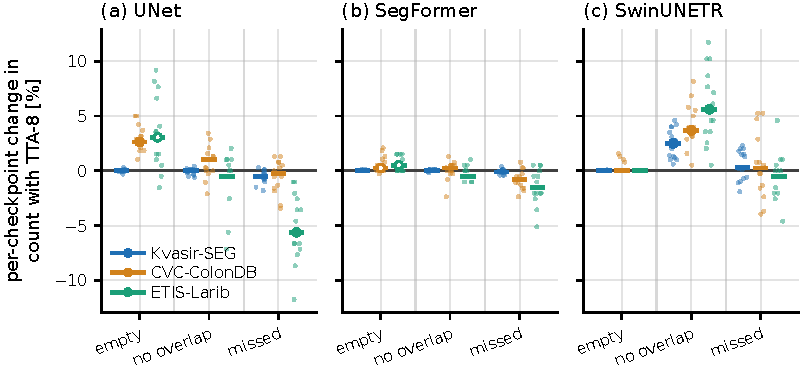
\includegraphics[width=\linewidth]{figures/fig_ckpt.pdf}}
\end{figure}

\emph{Per checkpoint.} With the checkpoint as the unit (Fig.~\ref{fig:ckpt}), 5 of the 27 cells survive Holm correction at $p<0.01$. Three are SwinUNETR's: images with no overlap rose in all 15 checkpoints on all three collections (medians $+25$, $+14$ and $+11$, Holm $p=0.002$ each) while its missed images moved in no direction on any of them (unadjusted $p=0.30$, $1.0$ and $0.39$), so within each collection, on the same predictions, one criterion says significantly harmed and the other says nothing. The other two are UNet's, and they point opposite ways in different collections: more images left empty on CVC-ColonDB in all 15 checkpoints (median $+10$ of 380) and fewer missed at IoU 0.10 on ETIS-Larib in all 15 (median $-11$ of 196). On ETIS-Larib alone UNet shows both directions at once, though only the fall survives correction, with empty predictions up in 13 of 15 checkpoints (median $+6$, $p=0.007$). SegFormer's empty predictions rose too, on CVC-ColonDB and ETIS-Larib (12 of 15 and 9 of 15, median $+1$ each, $p=0.003$ and $0.004$), short of Holm but invisible to the majority vote, which moves SegFormer by at most three images under any count, so the vote understates this model rather than inflating it. The counts below are the image-level view.

\emph{Empty predictions.} For UNet, TTA emptied predictions. On CVC-ColonDB and ETIS-Larib, the images that most UNet checkpoints left empty rose from 55 to 68 of 380 (unadjusted $p=0.002$, block bootstrap of the change $[7, 20]$) and from 5 to 18 of 196 ($p<0.001$, $[4, 23]$) with TTA-8 (Appendix~\ref{app:figs}, Fig.~\ref{fig:misses}). The counts vary widely between checkpoints (on ETIS-Larib the median left 12 images empty without TTA and 15 with it, ranges 1 to 29 and 5 to 42), so the majority vote is a summary and not the behaviour of one model. The 14 newly empty ETIS-Larib images fall into 9 runs of consecutive image numbers against 13 expected at random, so those images are probably not independent and this $p$-value is optimistic.

\emph{No overlap.} Most newly empty images already had no overlap with the polyp: of the 15 and 14 newly emptied, 12 and 11 already had none without TTA, and UNet's no-overlap counts stayed at 70 and 33, the rest being real losses of single images (Appendix~\ref{app:qualitative}). For SwinUNETR, which never predicted an empty mask on a polyp-free frame, they rose with TTA-8 from 18 to 43 of 1000 on Kvasir-SEG, from 73 to 99 on CVC-ColonDB and from 50 to 71 on ETIS-Larib ($p<0.001$ each; block bootstraps $[15, 36]$, $[16, 37]$ and $[12, 32]$), while its Dice rose by 0.006 to 0.009.

\begin{figure}[!t]
\floatconts
  {fig:sweep}
  {\caption{How the verdict on TTA depends on the bar. For each collection, the change in missed images with TTA-8 (as a percentage of the collection) against the IoU an image must reach to count as localised; 0 is the any-overlap criterion. Above the line TTA looks harmful, below it helpful. Filled markers: exact McNemar $p<0.01$, unadjusted (not Holm survivors, unlike Fig.~\ref{fig:ckpt}). Shaded band: between the last bar at which any rise is significant and the first at which none is. Counts for five of these nine thresholds are in Table~\ref{tab:criteria}.}}%
  {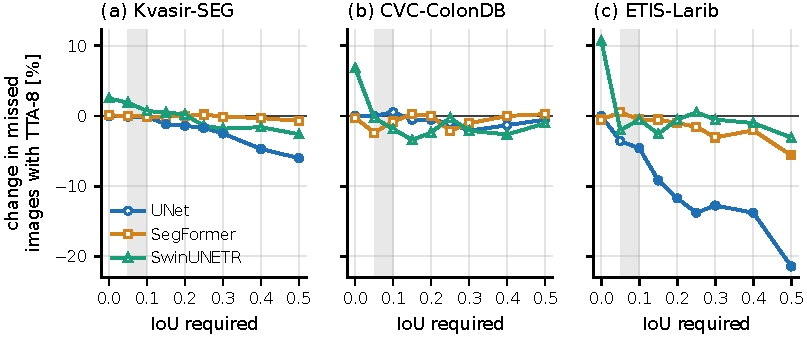
\includegraphics[width=\linewidth]{figures/fig_sweep.pdf}}
\end{figure}

\emph{Missed images.} With an IoU of at least 0.10 required, the SwinUNETR effect disappeared: missed images went from 216 to 223, 189 to 182 and 145 to 144 (the only rise at $p=0.37$; block bootstraps $[-6, 20]$, $[-21, 7]$ and $[-7, 4]$). That model had failed externally (Dice 0.14 to 0.40), and what it lost with TTA was mostly overlap that did not reach this IoU. UNet missed fewer images on ETIS-Larib with TTA-8, 46 against 55 (none newly missed, 9 recovered, $p=0.004$, $[-18, -2]$), and about as many on CVC-ColonDB (76 against 74; $[-2, 6]$) and Kvasir-SEG (26 against 27; $[-6, 3]$). SegFormer changed by at most three images under any of the three counts. The sweep says where in the grid the verdict turns (Fig.~\ref{fig:sweep}): requiring any overlap, three counts rise significantly, all SwinUNETR's; at IoU 0.05 one still does, SwinUNETR on Kvasir-SEG, a single unadjusted test on the broken model in the one collection we could not block, which we record and do not build on; from 0.10 upward none does, in any of the 63 comparisons at the seven thresholds from 0.10 to 0.50, the smallest $p$ on any rise being 0.37. We chose 0.10 after seeing the first two counts, so we cannot call it the right bar, only the lowest in our grid at which no rise survives anywhere. Above it the direction is stable and favours TTA, with UNet's falls on ETIS-Larib growing to 85 against 58 at 0.25 and 131 against 89 at 0.50 (Appendix~\ref{app:criteria}).

These are non-rejections, not demonstrations of safety: the widest interval admits about 20 more missed images per 1000, we set no non-inferiority margin, and the study was not powered to exclude a small rise. We hold the fall to the same bar we set for rises: it counts as a result because the direction repeats, at every threshold from 0.10 to 0.50 and in all 15 checkpoints, but it does not repeat across datasets, so it is a result about UNet on ETIS-Larib and not about TTA. These counts are also images and not polyps. On ETIS-Larib the 9 images UNet no longer missed fall into 7 runs of consecutive image numbers and the 14 newly empty images into 9 runs, so each stands on single-digit numbers of polyp episodes within a set holding 44 polyps, and the releases carry no polyp identities to resolve it further.

Gains by lesion size ran the other way from the losses, being smallest for UNet on the largest-polyp tertile of all three sets and negative for SwinUNETR on two of them, while the emptied predictions were not confined to the smallest polyps (Appendix~\ref{app:size}).




\subsection{Recovery rules and the operating point}
\label{sec:res-rules}
% Source: detection_rules/internal_misses.csv, external/*/misses_vs_tta8.csv,
% brats/misses.csv, brats/false_positive.csv (McNemar vs TTA-8), internal_paired.csv,
% external/*/paired.csv, brats/paired.csv; false_alarm/tables/false_alarm_all.csv.
Both rules filled most of the empty predictions and cost no mean Dice (Table~\ref{tab:rules}, Appendix~\ref{app:rules}). With either, most UNet checkpoints left 13 images empty on CVC-ColonDB and none on ETIS-Larib, against 55 and 5 without TTA and 68 and 18 with TTA-8, and missed images on CVC-ColonDB fell from 76 with TTA-8 to 52 and 65 ($p<0.001$ each). They change no non-empty mask, yet NSD fell by 0.002 to 0.008 and HD95 rose by 1.1 to 6.8\,px (Holm $p<0.01$), the survivorship effect of Section~\ref{sec:res-external} running in reverse.

The price is false alarms. The models, trained only on frames containing a polyp, fired on most polyp-free frames from another centre (Appendix~\ref{app:sanity}). On the 1009 normal cecum frames the share with a predicted polyp was 70.8\% for UNet and 96.4\% for SegFormer, which TTA-8 lowered to 56.5\% and 89.9\%; SwinUNETR marked a polyp on all 1009 frames with and without TTA, and TTA-8 only shrank the mask. This matches the downward shift of foreground probability that emptied predictions under shift: UNet's mean maximum probability on these frames fell from 0.74 to 0.59. These models never saw a frame without a polyp, so the mechanism acts on networks calibrated only on positives, and we cannot say the direction would transfer to a model trained with negative frames, which is what a deployed detector is. The rules push the rate back up, for UNet to 94.5\% and 89.5\%, and every count is monotone in $t$. The middle setting is the informative one: at $t=0.30$ the rule removed the whole empty-prediction rise, leaving 5 images empty on ETIS-Larib against 5 without TTA and 45 on CVC-ColonDB against 55, and still missed fewer images than the baseline on both sets (44 against 55 and 71 against 74), at 78.5\% false alarms against 70.8\%. That is far too high to deploy, but it is the one setting in our grid that pays for the empty predictions without giving back the gain in localisation. TTA and the rules therefore move UNet along a trade-off between empty predictions and false alarms (Fig.~\ref{fig:operating}), which for SegFormer appears only at the checkpoint level. Both rules fire on 90\% or more of normal frames, which leaves them a probe into the shape of that trade-off and not a deployable setting.

% Source: results/paper_checks/single_view_rule.csv, strict_overlap.csv, strict_overlap_transitions.csv, operating_curve.csv
% (scripts/paper_checks/single_view_rule.py; configs/cvc_clinicdb/unet_resnet50_baserules.yaml).
The lower threshold alone did not give this recovery. Applied to the single view, the rule with $t=0.20$ left no image empty on either set, but missed images barely moved, 73 and 55 against 74 and 55 without it, while firing on 96.4\% of polyp-free frames: on a single view the rule fills empty masks mostly off the polyp. The same rule on TTA-8 missed 65 and 41 at 89.5\% false alarms. After the rule a prediction is empty exactly when its maximum probability is below $t$, so each arm traces a detection curve through $t=0.5$, 0.4, 0.3 and 0.2. The arms are matched on false-alarm rate, which allows three of those four points, because the single view at $t=0.2$ (96.4\%) exceeds anything TTA-8 reaches (89.5\%). At every matched rate the two sat within one percentage point, with the sign of the gap depending on whether image-checkpoint pairs or majorities are counted, and we did not test it (Appendix~\ref{app:criteria}). We read this as consistent with a threshold change for empty outputs rather than evidence of one. The gain in missed images is separate, because it depends on where the mask lands, which a curve of whether the model outputs anything cannot measure.



\section{Discussion}
\label{sec:discussion}
% Sources: false_alarm/tables/false_alarm_all.csv (mean_max_prob); detection_rules/external/*/
% misses_vs_tta8.csv (left_vs_reference, new_vs_reference = 0); compare_models/gain_difference.csv;
% pass_latency.csv; aggregate_*/uncertainty_audit_*.csv and results/paper_checks (BraTS);
% Fan et al. 2020 (random 80/10/10 image split, mDice 0.899 on CVC-ClinicDB); workshop paper
% (UNSURE 2026): larger gains claimed for the lower-performing model; UNet dDice -0.0046;
% one from-scratch model vs pretrained ones; no baseline-error vs gain analysis.

\paragraph{TTA lowered foreground probability, and the count decides how that looks.} Averaging views pulls the foreground probability down where only some views are confident. For UNet it left more images empty in nearly every checkpoint, but most of those images had not been localised before, and by the IoU criterion UNet missed fewer on ETIS-Larib and about as many elsewhere. For SwinUNETR, images with no overlap rose in all 15 checkpoints on every external set while missed images did not: that model marked a polyp on every polyp-free frame with and without TTA, so what TTA took from it was mask area and not detections. For UNet and SegFormer, whose masks could disappear, false alarms on the cecum frames fell, the same shift seen from the other side. The clearest case is within one model on one set: on ETIS-Larib the same UNet checkpoints and images give three answers, with empty predictions up from 5 to 18, no-overlap images unchanged at 33, and missed images down from 55 to 46. A study reporting only the first would conclude that TTA harms UNet. For empty outputs TTA sat close enough to the single view's detection curve that we could not separate them, so a threshold change is a plausible reading there; the lower count of missed images is not explained that way, because it depends on where the mask lands.

\paragraph{Where the effect appears.} Mostly, but not only, in models already failing. By the majority vote SegFormer changed by at most three images under each count on every set, and dropping SwinUNETR, which we broke on purpose, would leave a single two-way disagreement on ETIS-Larib. Per checkpoint the base is wider: the disagreement holds for SwinUNETR within all three collections, for UNet across two, and SegFormer's empty predictions rise on two before correction. The effect is still largest where the model is weakest, which narrows the claim without removing it, because a pre-deployment check is run precisely where a model may be weak or shifted.

\paragraph{Clinical reading.} Both errors have a clinical cost. A higher adenoma detection rate is linked to less interval cancer \cite{corley2014adr}, but that evidence is per endoscopist and not per frame, so our data cannot weigh one error against the other. For UNet on ETIS-Larib, TTA left about 66 more images per 1000 empty while missing about 46 fewer; the false alarms it removed were counted on other frames in another hospital, so those are separate observations and not one trade. A frame on which the system goes quiet still gives no prompt, so empty predictions deserve their own count even when the removed prediction was wrong. Eight views took about 298\,ms per frame at batch 1, so in this form TTA suits offline use rather than live video, though batching could change that and we did not measure it. Two points follow. Report misses with an explicit localisation criterion, next to empty predictions and false alarms, whenever the inference procedure changes, since any single rule would have settled the verdict here by itself. And check empty predictions separately, because no ROI signal can score them.

\paragraph{Limitations.} This is a retrospective study on public data, with no reader study and no patient-level outcome. The central negative result is a failure to detect harm, not a demonstration of safety: no non-inferiority margin, no power for one, and intervals still admitting about 20 more missed images per 1000. The 15 checkpoints are 5 folds $\times$ 3 seeds from one recipe on one collection and not independent replicates, so every test here describes this pool. We count misses per image, so a missed frame is not a missed polyp, and image-level IoU is not a clinical standard, is harder to reach for small polyps and ignores images with several polyps; we added that criterion after seeing the any-overlap counts and swept it on the data that motivated it. A false alarm is any non-empty mask, the cecum frames carry an anatomical-landmark label from one hospital, and the ET-free population is 33 patients. All 2D models come from one small single-centre collection, no external collection carries centre or sequence labels, and the external evidence rests on well under 100 patients; PolypGen \cite{ali2023polypgen} would permit a cluster-correct, multi-centre analysis. We did not analyse calibration or re-threshold non-empty predictions, so missed images are compared at matched thresholds and not at matched false-alarm rates, and part of the external distance gain may be survivorship. The pattern rests on three models, one failed by design; the uncertainty audit is internal only; and we studied geometric TTA only.

\section{Conclusion}
\label{sec:conclusion}
Geometric TTA raised Dice everywhere lesions were present, but whether it lost lesions under shift depended on how a miss was counted: on the same predictions and the same checkpoints, one criterion called a model significantly harmed while another found nothing. We found no significant net loss of lesions the models still placed on target, within intervals wide enough to hide one. Seeing any of it needed external and polyp-free data and three miss counts beside Dice, reported per checkpoint rather than as one vote, which we recommend whenever an inference procedure changes.


\clearpage % references and appendix do not count

\bibliography{refs}

\appendix
% Appendix: does not count toward the page limit.

\section{Training and inference details}
\label{app:training}
All 2D models were trained with an equally weighted sum of binary cross-entropy and Dice loss, AdamW (learning rate $10^{-4}$, no weight decay), a cosine schedule, at most 100 epochs and mixed precision, with batch size 8 (4 for SwinUNETR). Input size was $352\times352$. Training augmentation was a random rotation by a multiple of 90$^\circ$, horizontal and vertical flips (each $p=0.5$), and brightness and contrast scaling by factors in $[0.85, 1.15]$ on the raw image. Pretrained encoders used ImageNet normalisation and SwinUNETR used per-fold dataset statistics. We kept the checkpoint with the best Dice on the validation fold and stopped after 20 epochs without improvement. The test fold was never used during training or selection.

The 3D SegResNet used the four MRI sequences (FLAIR, T1, T1-Gd, T2), each clipped at its 1st and 99th brain percentiles and z-scored over brain voxels. Training used the same loss, optimiser and schedule, $128^3$ patches from the brain bounding box, 90\% of them centred on an enhancing-tumour voxel (250 per epoch), at most 100 epochs with patience 20 on Dice over 40 validation-fold patients, and flips on all three axes, axial 90$^\circ$ rotations and intensity jitter of $\pm0.1$ as augmentation. Inference used sliding windows of $128^3$ with overlap 0.5 and Gaussian weighting.

We measured per-pass latency on a laptop GPU (NVIDIA RTX 4050, batch 1, mixed precision, $352\times352$): 10 warm-up passes, then the median of three blocks of 50 passes. TTA latency is estimated as passes times the per-pass median.


The six uncertainty signals of Section~\ref{sec:eval} are: the mean predictive entropy in the ROI for the single view and for the TTA-4 mean map, the mean TTA-4 variance in the ROI, one minus the mean probability inside the predicted mask, the fraction of pixels on which the binarised views do not all agree, and one minus the mean pairwise Dice between views. The ROI is the predicted foreground plus a 3-pixel band around it. The third failure definition compares empty predictions against clean cases, meaning non-empty predictions with Dice at least 0.5.

\paragraph{Statistical detail from Section~\ref{sec:eval}.} Bootstrap intervals use 10{,}000 draws, reduced to 2{,}000 for between-model gain comparisons and MC-Dropout and 1{,}000 for the uncertainty audit and its paired tests. External rates of empty predictions carry Jeffreys intervals. For tails we report the 90th percentile of HD95 and the large-failure rate with bootstrap intervals of the change. Gains across models are compared as the absolute change, the share of remaining error recovered ($\Delta\mathrm{Dice}/(1-\mathrm{Dice}_{\text{base}})$, computed per video then averaged) and the log ratio of HD95; because a plain correlation between baseline error and gain is biased by regression to the mean, we use Oldham's method \cite{oldham1962} against a permutation null that exchanges baseline and TTA scores within whole videos. Counts per checkpoint are descriptive.

\section{Further internal comparisons}
\label{app:further}
% Source: aggregate_*/ensemble_comparison.csv; mc_dropout_cvc_clinicdb_unet_resnet50_dropout/deltas.csv.
\paragraph{Large failures and the extreme tail (internal).} TTA-4 cut the share of frames with HD95 above 50\,px, or with no prediction from any seed, from 41.0\% to 31.0\% for UNet (95\% CI $[-15.0, -5.4]$ points) and from 27.8\% to 25.7\% for SegFormer, while neither 90th percentile of HD95 moved reliably ($-10.3$\,px $[-25.4, 2.3]$ and $-4.0$\,px $[-14.4, 11.4]$). For SwinUNETR and BraTS the upper tail did shrink, by 9.0\,px $[-14.6, -1.4]$ and 1.5\,mm $[-3.0, -0.3]$, and on BraTS large failures fell from 11.9\% to 10.7\% $[-2.1, -0.3]$. HD95 percentiles use each method's own non-empty cases.

A three-seed deep ensemble was not significantly better than TTA-4 of a single model. The Dice difference was +0.003 for UNet, +0.004 for SegFormer and +0.006 for SwinUNETR, with Holm $p=1.0$ in each case. Combining the two added 0.013, 0.007 and 0.018 Dice over TTA-4 ($p<0.001$). MC-Dropout with eight passes was, if anything, slightly worse than the deterministic pass of the same network (Dice $-0.001$, unadjusted 95\% CI $[-0.002, -0.0001]$, Holm $p=0.13$) and stayed 0.022 below TTA-4 of that network (Holm $p<0.001$).

% Source: compare_data_sweep/deltas.csv and gain_difference.csv (seed 0 only); compare_models/residual_error.csv.
% Source: compare_models/gain_difference.csv (TTA-4, paired by video, unadjusted p); compare_models/residual_error.csv.
In absolute Dice, the two weaker models gained numerically more than the strongest: UNet (+0.023) gained more than the stronger SegFormer (+0.011; difference 0.012, 95\% CI $[0.003, 0.021]$, $p=0.002$) and about as much as the weaker SwinUNETR (+0.021; $p=0.37$). Relative to what was left to gain, the mid-quality UNet gained most. As a share of the remaining error, computed per video and then averaged so that it differs from the ratio of the means in Table~\ref{tab:internal}, UNet closed 13.0\%, SegFormer 7.1\% and SwinUNETR 6.3\%, and UNet's share was larger than both ($p=0.004$ and $p=0.006$). HD95 followed the same pattern on a log scale: $-0.39$ for UNet against $-0.11$ for both other models ($p<0.001$).

Within UNet, less training data did not raise the gain. With 100\%, 50\% and 25\% of the training videos (5 folds at one seed, so the 100\% arm's 0.028 is not Table~\ref{tab:internal}'s 0.023), TTA-4 added 0.028, 0.026 and 0.014 Dice; the last was not significant (Holm $p=0.07$), and no two fractions differed in Dice gain ($p\geq0.55$). Within each model, harder cases did not consistently gain more. With Oldham's correction, the correlation between a case's mean score and its Dice gain was $-0.11$ for UNet (permutation $p=0.16$), $-0.15$ for SegFormer ($p=0.08$) and $+0.17$ for SwinUNETR ($p=0.04$), where it was the better cases that gained more.

The workshop study reported larger TTA gains for a lower-performing model \cite{kashyap2026unsure}, based on one model trained from scratch against pretrained ones and without relating baseline error to gain. Here the mid-quality UNet gained more than the stronger SegFormer (0.023 against 0.011, $p=0.002$), and the weaker SwinUNETR did not gain significantly more than UNet (0.021, $p=0.37$) and recovered a smaller share of its error. The workshop UNet showed no Dice gain ($-0.005$), while the retrained UNet here gains 0.023, so the two studies are not directly comparable.


\section{Additional result figures}
\label{app:figs}

\begin{figure}[htbp]
\floatconts
  {fig:misses}
  {\caption{Empty predictions without TTA, with TTA-4 and with TTA-8 (grey shades). (a) Internal: share of cases with an empty prediction (CVC-ClinicDB frames empty in at least 2 of 3 seeds; BraTS patients), with 95\% cluster-bootstrap intervals and Holm-adjusted McNemar $p$. (b) UNet and (c) SegFormer on the external sets: share of images left empty by at least 8 of 15 checkpoints, with 95\% Jeffreys intervals and exact McNemar $p$ (unadjusted). SwinUNETR left no external image empty by majority. No-overlap and missed counts are in Table~\ref{tab:external}.}}
  {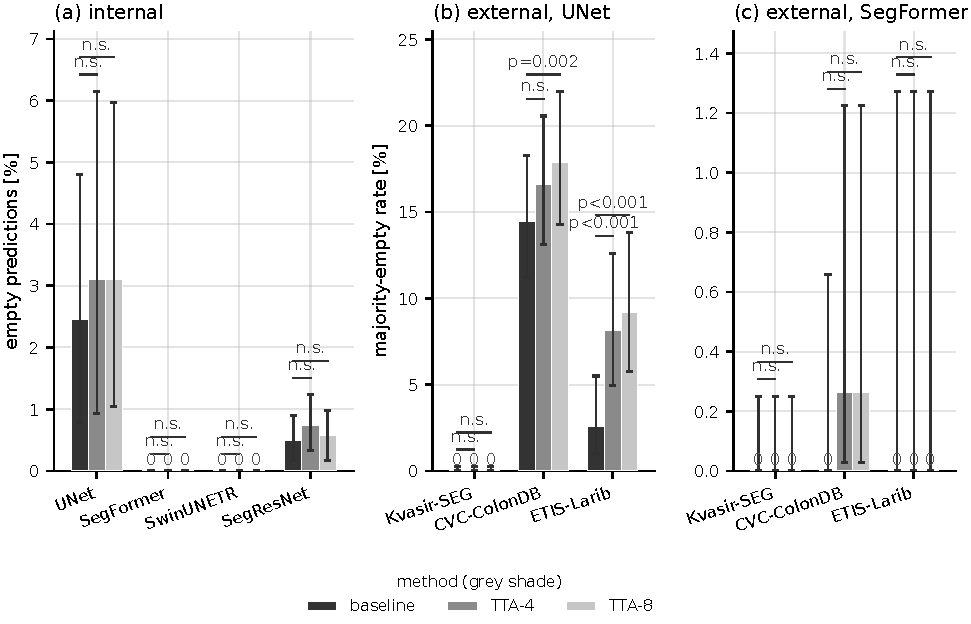
\includegraphics[width=\linewidth]{figures/fig03_misses.pdf}}
\end{figure}

These figures show results that the main text reports in numbers: the risk--coverage curves of Section~\ref{sec:res-uncertainty} (Fig.~\ref{fig:riskcov}), the gain against the number of views of Section~\ref{sec:res-internal} (Fig.~\ref{fig:views}), the HD95 distribution of Section~\ref{sec:res-failures} (Fig.~\ref{fig:ecdf}) and the gain against domain gap of Section~\ref{sec:res-external} (Fig.~\ref{fig:external}).

Three further numbers from the uncertainty audit of Section~\ref{sec:res-uncertainty}. On BraTS the TTA-4 variance in the ROI was the best signal (AUROC 0.96, against 0.90 for ROI entropy, $p<0.002$), while view disagreement ranked failures there as more certain than successes (0.36). Pairwise Dice between views, computed for UNet only, scored higher than view disagreement on the empty frames (0.71 against 0.21, 19 frames), but its 95\% CI $[0.50, 0.95]$ reaches chance.

Why view disagreement fails on empty predictions: an empty prediction has almost no pixels on which views can disagree, because the score of Section~\ref{sec:eval} is a fraction of all image pixels and is not normalised by predicted area, while the boundary of a large, correctly segmented lesion adds many pixels. A version normalised by predicted area plus band would be the natural repair, and it needs no retraining; we did not compute one, so we report the defect rather than a fix.

\begin{figure}[htbp]
\floatconts
  {fig:riskcov}
  {\caption{Risk--coverage curves of five uncertainty signals, UNet on CVC-ClinicDB, each scored against the failures of its own prediction: (a) Dice $<0.5$ on a non-empty prediction, (b) the same plus empty predictions; ROI-based signals are undefined on the 14 frames with no prediction from any seed and exclude them. Cases are kept from the most confident; the curve shows the failure rate of the kept cases. The two numbers after each signal in the legend are its AUROC and its AURC, the latter with risk $=1-$Dice.}}
  {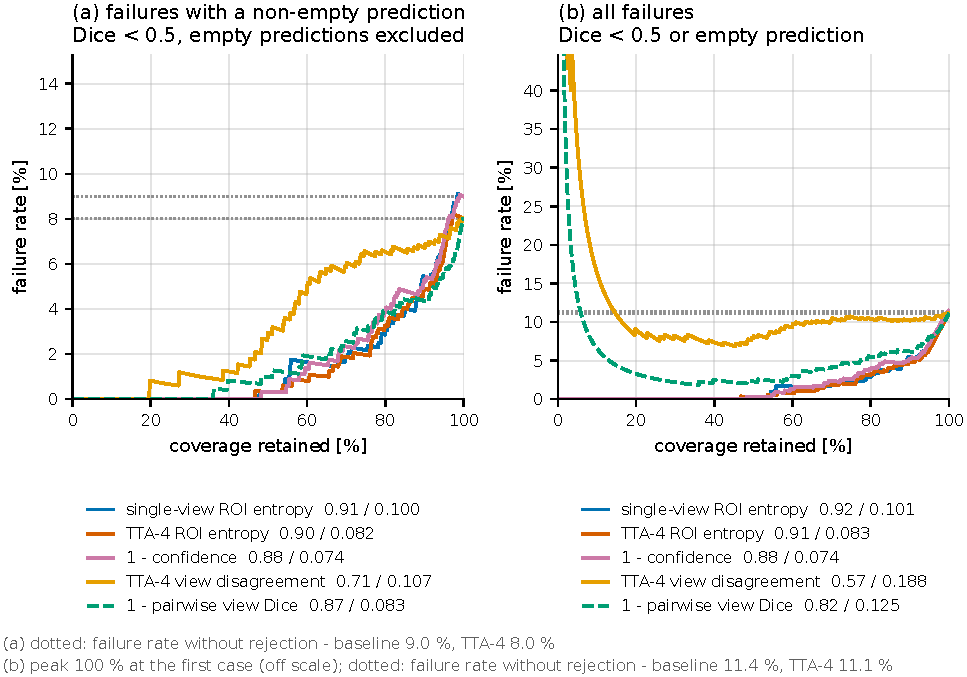
\includegraphics[width=\linewidth]{figures/fig05_risk_coverage.pdf}}
\end{figure}

\begin{figure}[htbp]
\floatconts
  {fig:views}
  {\caption{Change against the single view for 1, 2, 4 and 8 views: (a) Dice, (b) relative HD95 change, for every internal and external setting (colour: dataset; line style and marker: model). Error bars: 95\% bootstrap intervals of the paired per-case change. Small horizontal offsets separate overlapping lines.}}
  {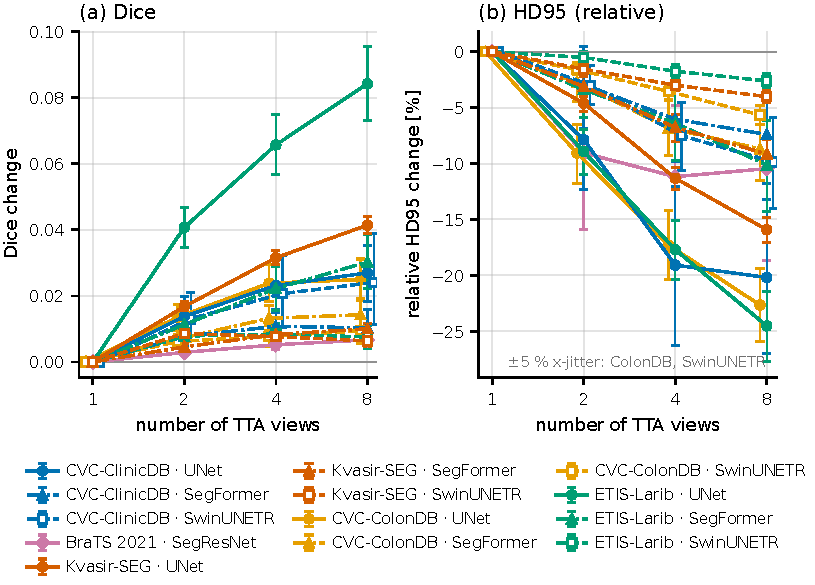
\includegraphics[width=\linewidth]{figures/fig01_gain_vs_views.pdf}}
\end{figure}

\begin{figure}[htbp]
\floatconts
  {fig:ecdf}
  {\caption{ECDF of per-frame HD95 (mean over 3 seeds; frames non-empty under both methods), UNet on CVC-ClinicDB, baseline vs TTA-4. Dashed line: 50\,px; dotted lines: 95th percentiles. Rates printed in the panel exclude empty predictions, so they differ from the text.}}
  {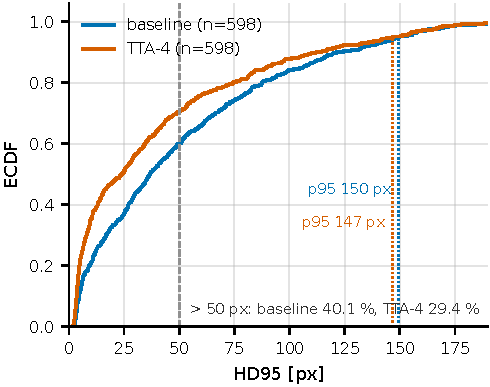
\includegraphics[width=0.6\linewidth]{figures/fig04_hd95_ecdf.pdf}}
\end{figure}

\begin{figure}[htbp]
\floatconts
  {fig:external}
  {\caption{Absolute TTA-8 Dice gain against domain gap, the relative drop of an external collection's baseline Dice below the architecture's internal frame-level baseline. Points at zero gap and dashed lines: internal CVC-ClinicDB gains. These internal gains are frame-level TTA-8 means (UNet 0.028, SwinUNETR 0.021, SegFormer 0.011), not the video-level TTA-4 values of Table~\ref{tab:internal}, so they do not match that table. Error bars: 95\% cluster bootstrap intervals (one image per cluster externally, one video internally).}}
  {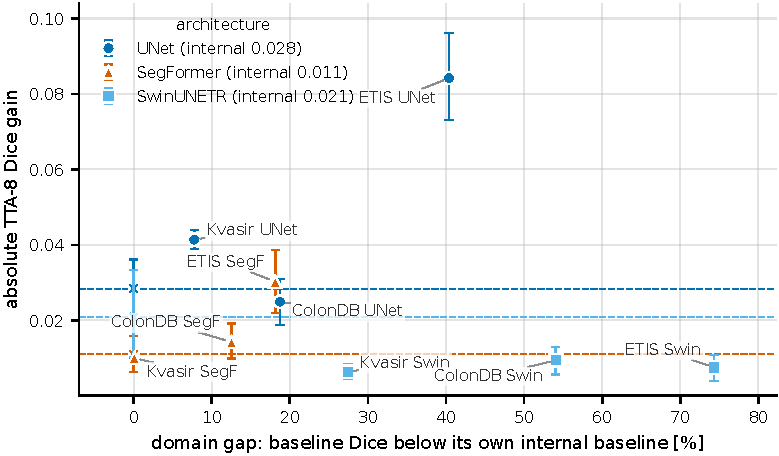
\includegraphics[width=\linewidth]{figures/fig02_internal_vs_external.pdf}}
\end{figure}


\paragraph{The single-view detection curve.} The three comparable rates of Section~\ref{sec:res-rules} in full. At the single view's false-alarm rates of 70.8\%, 75.6\% and 84.8\% ($t=0.5$, 0.4, 0.3), its share of empty predictions over image-checkpoint pairs on CVC-ColonDB and ETIS-Larib was 11.7\%, 10.5\% and 7.2\%, against 11.3\%, 9.9\% and 6.6\% for TTA-8 linearly interpolated between its neighbouring thresholds at those same rates. Counted by a majority of checkpoints the order reverses at two of the three rates and ties at the third: 10.4\%, 9.4\% and 4.3\% against 10.6\%, 9.4\% and 5.0\%. The sweep moves only the empty-versus-non-empty decision; we did not re-threshold non-empty predictions.

\section{Miss counts under different criteria}
\label{app:criteria}
% Source: results/paper_checks/strict_overlap.csv, strict_overlap_transitions.csv, per_checkpoint_spread.csv,
% miss_clustering.csv (scripts/paper_checks/robustness_checks.py).
Table~\ref{tab:criteria} repeats the external counts of Table~\ref{tab:external} for IoU thresholds from 0 (no overlap) to 0.50. A rise that is significant appears only at 0, where all three SwinUNETR counts rise, and at 0.05, where SwinUNETR on Kvasir-SEG still does (125 to 144). From 0.10 upward no count rose significantly for any model on any set. Several fell: for UNet on ETIS-Larib the fall is numerical at 0.05 and significant at every threshold from 0.10 upward, and on Kvasir-SEG it is significant at 0.25 and 0.50. Counted per checkpoint, SwinUNETR's predictions with no overlap rose in all 15 checkpoints on every set (median change $+25$, $+14$ and $+11$ predictions), while its predictions with IoU below 0.10 rose in 10, 8 and 4 checkpoints and fell in 5, 7 and 8 (3 unchanged on ETIS-Larib). For UNet on ETIS-Larib, predictions with IoU below 0.10 fell in all 15 checkpoints (median $-11$). External images carry no sequence labels. As a rough check of independence we grouped the newly affected images into runs of consecutive image numbers and compared the number of runs with random placement (10,000 permutations). The 14 newly empty UNet images on ETIS-Larib formed 9 runs against 13.1 expected ($p=0.001$), and the 27 SwinUNETR images that newly lost overlap on CVC-ColonDB formed 21 runs against 25.2 ($p=0.006$); the 15 newly empty UNet images on CVC-ColonDB formed 15 runs. The 9 ETIS-Larib images that UNet no longer missed under the IoU criterion formed 7 runs against 8.6 expected ($p=0.045$), so they are not fully independent either.

We therefore repeated every external comparison with a block bootstrap. Images are cut into contiguous blocks of consecutive image numbers, with the block length set to the mean sequence length reported for the collection (CVC-ColonDB: 380 images over the 15 sequences its release describes, so 25, although that sequence count belongs to the 300-frame release and not to the 380-frame split we use; ETIS-Larib: 196 in 34, so 6; Kvasir-SEG carries no released sequence labels and we did not block it, so its intervals resample images), and blocks are resampled with replacement 10,000 times. Other bootstrap intervals in this paper use 10,000 draws, reduced to 2,000 for between-model gain comparisons and MC-Dropout and 1,000 for the uncertainty audit and its paired tests. The blocks stand in for sequences; they are not the real ones, real sequences are not of equal length, and on CVC-ColonDB there are only about 15 of them, so the effective sample size is small and these intervals are a sensitivity check rather than a cluster-correct analysis. No conclusion changed, which we read as a sign that the block structure recovers little of the real clustering rather than as evidence that clustering is absent. The intervals of the change exclude zero exactly where the image-level tests were significant: UNet empty predictions $[7, 20]$ on CVC-ColonDB and $[4, 23]$ on ETIS-Larib, SwinUNETR images with no overlap $[15, 36]$, $[16, 37]$ and $[12, 32]$, and the fall in UNet missed images on ETIS-Larib $[-18, -2]$. They include zero everywhere the image-level tests were not significant, including every missed count for SwinUNETR ($[-6, 20]$, $[-21, 7]$ and $[-7, 4]$) and for UNet on CVC-ColonDB ($[-2, 6]$).

\begin{table}[htbp]
\floatconts
  {tab:criteria}%
  {\caption{External images counted as missed by at least 8 of 15 checkpoints, baseline $\rightarrow$ TTA-8, for IoU below the threshold in the column head; 0 means no overlap (Dice $=0$). We swept nine thresholds (0, 0.05, 0.10, 0.15, 0.20, 0.25, 0.30, 0.40, 0.50) and show five here; the four omitted ones are monotone between their neighbours and change no conclusion. $^{\dagger}$exact McNemar $p<0.01$ (unadjusted); the direction is given by the arrow.}}%
  {
  \begin{tabular}{@{}llccccc@{}}
  \toprule
  Data & Model & 0 & 0.05 & 0.10 & 0.25 & 0.50 \\
  \midrule
  \multirow{3}{*}{Kvasir} & UNet & 1$\rightarrow$1 & 9$\rightarrow$8 & 27$\rightarrow$26 & 109$\rightarrow$92$^{\dagger}$ & 310$\rightarrow$250$^{\dagger}$ \\
   & SegFormer & 0$\rightarrow$1 & 5$\rightarrow$5 & 10$\rightarrow$9 & 27$\rightarrow$29 & 120$\rightarrow$113 \\
   & SwinUNETR & 18$\rightarrow$43$^{\dagger}$ & 125$\rightarrow$144$^{\dagger}$ & 216$\rightarrow$223 & 501$\rightarrow$487 & 862$\rightarrow$836$^{\dagger}$ \\
  \midrule
  \multirow{3}{*}{ColonDB} & UNet & 70$\rightarrow$70 & 72$\rightarrow$72 & 74$\rightarrow$76 & 92$\rightarrow$88 & 134$\rightarrow$132 \\
   & SegFormer & 12$\rightarrow$11 & 31$\rightarrow$22 & 36$\rightarrow$33 & 55$\rightarrow$47 & 94$\rightarrow$95 \\
   & SwinUNETR & 73$\rightarrow$99$^{\dagger}$ & 147$\rightarrow$146 & 189$\rightarrow$182 & 279$\rightarrow$278 & 354$\rightarrow$350 \\
  \midrule
  \multirow{3}{*}{ETIS} & UNet & 33$\rightarrow$33 & 47$\rightarrow$40 & 55$\rightarrow$46$^{\dagger}$ & 85$\rightarrow$58$^{\dagger}$ & 131$\rightarrow$89$^{\dagger}$ \\
   & SegFormer & 8$\rightarrow$7 & 14$\rightarrow$15 & 17$\rightarrow$16 & 31$\rightarrow$28 & 59$\rightarrow$48$^{\dagger}$ \\
   & SwinUNETR & 50$\rightarrow$71$^{\dagger}$ & 129$\rightarrow$125 & 145$\rightarrow$144 & 170$\rightarrow$171 & 192$\rightarrow$186 \\
  \bottomrule
  \end{tabular}}
\end{table}


\section{Recovery rules in full}
\label{app:rules}

\begin{figure}[!t]
\floatconts
  {fig:operating}
  {\caption{UNet's operating point without TTA, with TTA-4 and TTA-8, and with the recovery rules (markers): false-alarm rate on 1009 polyp-free cecum frames against the share of images left empty by at least 8 of 15 checkpoints on CVC-ColonDB and ETIS-Larib pooled (576 images). Solid line: TTA-8 with thresholds 0.5 to 0.2. Dashed line with open markers: the single view with the same thresholds. SegFormer is not plotted because almost none of its images are empty by majority. Every point sits above 50\% per-frame false alarms, so this compares inference procedures and is not a deployment curve. Missed images are in Table~\ref{tab:rules}.}}
  {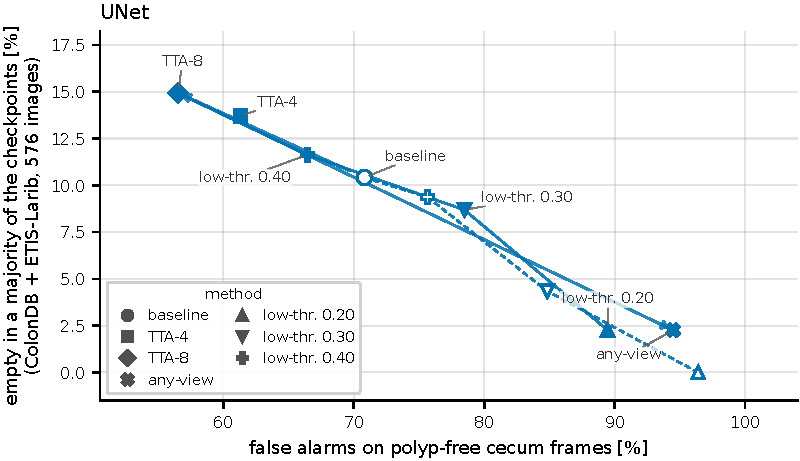
\includegraphics[width=\linewidth]{figures/fig08_operating_point.pdf}}
\end{figure}


Section~\ref{sec:res-rules} reports these numbers in the text. The rules are a probe into the shape of the trade-off and not a deployable setting: both fire on 90\% or more of polyp-free frames.

\begin{table}[htbp]
\floatconts
  {tab:rules}%
  {\caption{Empty predictions, missed images and false alarms, UNet (CVC) and SegResNet (BraTS). The rules are applied to TTA-8, and in the last row to the single view ($-$ = not run). Empty: majority of checkpoints (external), $\geq$2 of 3 seeds (internal), per patient (BraTS). Missed (IoU $<0.10$): majority of checkpoints. False alarms: share of 1009 polyp-free HyperKvasir cecum frames with a non-empty prediction (mean over 15 checkpoints); BraTS: patients of 33 without enhancing tumour (ET-free) with any predicted enhancing tumour. $^{*}$The threshold $t$ was chosen on these data (in-sample).}}%
  {
  \begin{tabular}{@{}lcccccccc@{}}
  \toprule
  Method & \multicolumn{4}{c}{Empty} & \multicolumn{2}{c}{Missed} & \multicolumn{2}{c}{False alarms} \\
  \cmidrule(lr){2-5}\cmidrule(lr){6-7}\cmidrule(lr){8-9}
   & CVC & ColonDB & ETIS & BraTS & ColonDB & ETIS & Cecum & BraTS \\
   & (612) & (380) & (196) & (1218) & (380) & (196) & frames & (33) \\
  \midrule
  Baseline            & 15 & 55 & 5  & 6 & 74 & 55 & 70.8\% & 22 \\
  TTA-8               & 19 & 68 & 18 & 7 & 76 & 46 & 56.5\% & 21 \\
  Any-view            & 5  & 13 & 0  & 0 & 52 & 42 & 94.5\% & 32 \\
  Low-thr. 0.20       & 8$^{*}$ & 13 & 0 & 0 & 65 & 41 & 89.5\% & 30 \\
  Low-thr. 0.30       & 14 & 45 & 5 & 3 & 71 & 44 & 78.5\% & 27 \\
  Low-thr. 0.40       & 17 & 53 & 14 & 5 & 73 & 46 & 66.4\% & 24 \\
  Single view 0.20    & $-$ & 0 & 0 & $-$ & 73 & 55 & 96.4\% & $-$ \\
  \bottomrule
  \end{tabular}}
\end{table}

\section{Lesion-size subgroups}
\label{app:size}
% Source: external_by_model/subgroup_delta.csv, subgroup_interaction.csv, subgroup_summary.csv (TTA-8 vs baseline).
For UNet, the TTA-8 Dice gain differed between size tertiles on all three external collections (Kruskal--Wallis, Holm $p\leq0.03$). On Kvasir-SEG it fell with polyp size (0.061, 0.040 and 0.023 from the smallest to the largest tertile), and on CVC-ColonDB the gain for the largest polyps was small (0.005, 95\% CI $[-0.007, 0.016]$). SwinUNETR lost Dice on the largest polyps of Kvasir-SEG and CVC-ColonDB ($-0.003$ and $-0.008$). SegFormer's gain did not differ between tertiles on CVC-ColonDB or ETIS-Larib (Holm $p=1.0$). The images left empty by most UNet checkpoints rose in every tertile: on CVC-ColonDB from 23 to 30, 12 to 13 and 20 to 25 in the small, medium and large tertiles, and on ETIS-Larib from 4 to 10, 1 to 5 and 0 to 3 (counts, not tested per tertile; Section~\ref{sec:res-external}); SwinUNETR left no image empty by majority in any tertile (Fig.~\ref{fig:size}).
\begin{figure}[htbp]
\floatconts
  {fig:size}
  {\caption{Size tertiles of reference polyp area, cut per external collection (Kvasir-SEG at 25{,}204 and 55{,}261\,px; CVC-ColonDB at 7{,}471 and 16{,}726\,px; ETIS-Larib at 13{,}723 and 49{,}260\,px). Top: TTA-8 Dice gain with 95\% bootstrap intervals for (a) UNet, (b) SegFormer and (c) SwinUNETR. Bottom: share of images left empty by at least 8 of 15 checkpoints without TTA (open markers) and with TTA-8 (filled).}}
  {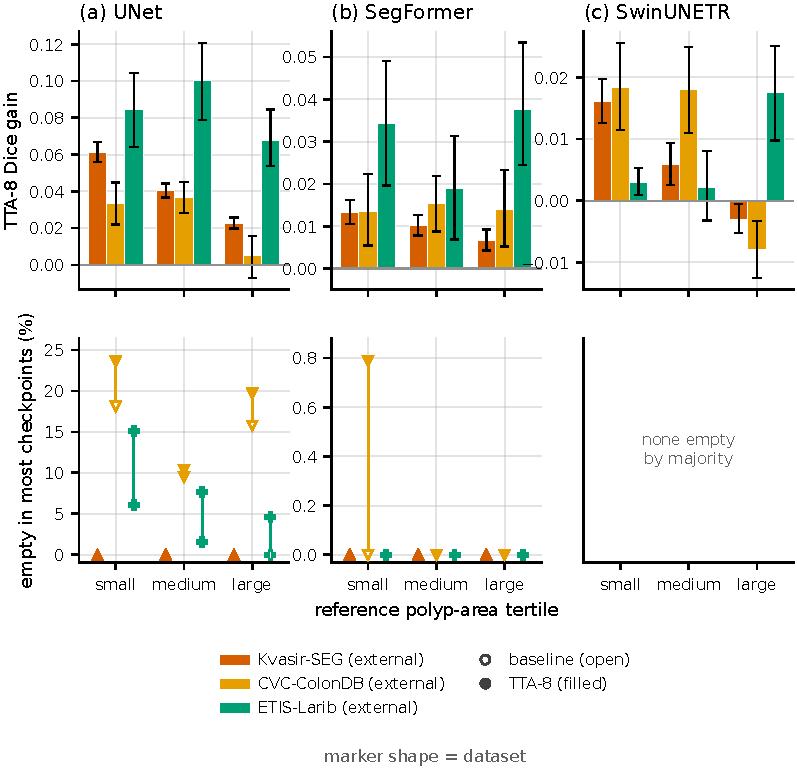
\includegraphics[width=\linewidth]{figures/fig06_size_subgroups.pdf}}
\end{figure}

\section{Qualitative examples}
\label{app:qualitative}
% Source: scripts/figures/fig07_qualitative.py (selection rule, recomputation, Dice assertion).
Rows in Fig.~\ref{fig:qualitative} were chosen by a fixed rule, not by eye. An external row qualifies when most of the 15 checkpoints give a non-empty prediction without TTA and most give an empty one with TTA-8. The internal rows are the two CVC-ClinicDB frames with the largest TTA-4 Dice gain averaged over seeds. The maps of each row were recomputed with the stated checkpoint through the evaluation code, and the Dice printed for each row was checked against the evaluation table (tolerance 0.011).

\begin{figure}[htbp]
\floatconts
  {fig:qualitative}
  {\caption{Top three rows: external polyps (CVC-ColonDB, ETIS-Larib) on which most of the 15 checkpoints give a non-empty prediction without TTA and most an empty one with TTA-8. Bottom two rows: internal CVC-ClinicDB frames with the largest TTA-4 Dice gain averaged over seeds, each drawn with the checkpoint showing the largest gain. External rows are drawn with a checkpoint in which the TTA-8 prediction is empty and the baseline Dice is at least 0.3, smallest polyps first; the Dice of each row is printed next to it. The external rows show individual losses, which are the minority among newly empty images; Table~\ref{tab:external} gives net counts.}}
  {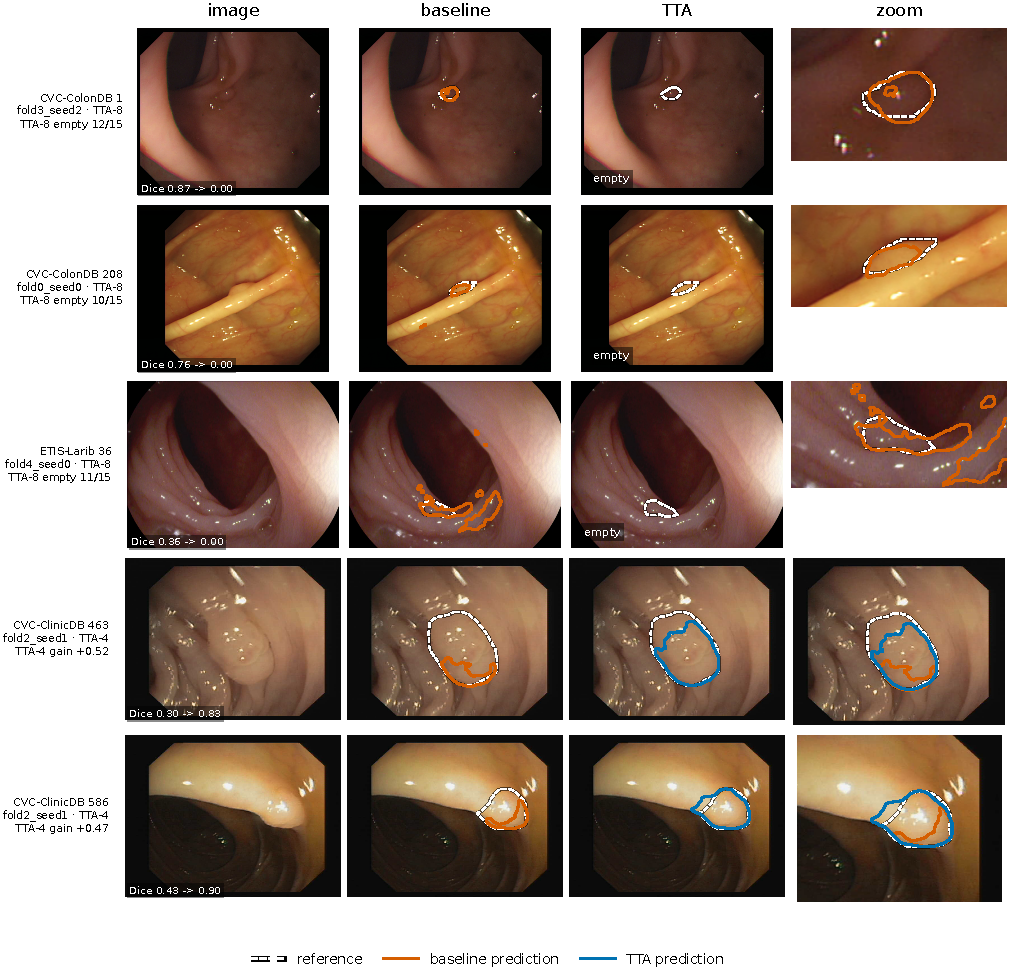
\includegraphics[width=\linewidth]{figures/fig07_qualitative.pdf}}
\end{figure}

\section{False alarms on polyp-free frames}
\label{app:sanity}
% Source: scripts/figures/sanity_false_alarms.py (seeded draw, CPU recomputation, region attribution,
% preprocessing assertion against the Kvasir-SEG loader).
To rule out a pipeline artefact behind the high false-alarm rates, we drew baseline false alarms at random (fixed seed) from the fold-0, seed-0 UNet and SegFormer runs, recomputed them on the CPU through the evaluation code, and assigned every predicted region to what it covers: mucosa, the black border, the endoscope overlay box or the overlay text. All twelve shown lie on mucosa (Fig.~\ref{fig:sanity}). A numerical check confirmed that the polyp-free frames pass through the same preprocessing as Kvasir-SEG, giving the same network input for the same image file.

\begin{figure}[htbp]
\floatconts
  {fig:sanity}
  {\caption{Twelve baseline false alarms on HyperKvasir normal cecum frames, drawn at random with a fixed seed from one checkpoint pair (fold 0, seed 0): eight UNet (blue) and four SegFormer (vermillion). All twelve lie on mucosa, none on the overlay box, border or text.}}
  {\includegraphics[width=\linewidth]{figures/sanity_false_alarms.png}}
\end{figure}

\section{Effects per 1000 cases and latency}
\label{app:deployment}
% Source: aggregate_*/tail_metrics.csv and detection_seed_averaged.csv (internal), results/paper_checks/
% brats_tail_et_only.csv (BraTS, 1218 ET patients), external_by_model/misses.csv (external, majority of 15
% checkpoints), deployment_terms/pass_latency.csv (2D latency). No BraTS latency: no measurement record.
Table~\ref{tab:deployment} restates the main effects per 1000 cases. Large failures fixed is the drop in the share of cases with HD95 above 50\,px (CVC-ClinicDB) or 10\,mm (BraTS) or with no prediction. Empty added is the net change in empty cases, by majority of seeds (internal) or of the 15 checkpoints (external). SwinUNETR lost all overlap on 25, 68 and 107 more images per 1000 on Kvasir-SEG, CVC-ColonDB and ETIS-Larib, but by the IoU criterion no model missed significantly more images (Table~\ref{tab:criteria}). Latency is estimated as the number of views times the measured median per-pass time.

\begin{table}[htbp]
\floatconts
  {tab:deployment}%
  {\caption{Effects per 1000 cases and estimated latency per image (-- = not measured). External settings not listed added no empty predictions by majority (Kvasir-SEG for every model; SegFormer on ETIS-Larib; SwinUNETR everywhere).}}%
  {
  \begin{tabular}{lcccccc}
  \toprule
  Setting & \multicolumn{2}{c}{Large failures fixed} & \multicolumn{2}{c}{Empty added} & \multicolumn{2}{c}{Latency (ms)} \\
  \cmidrule(lr){2-3}\cmidrule(lr){4-5}\cmidrule(lr){6-7}
   & TTA-4 & TTA-8 & TTA-4 & TTA-8 & 1 view & TTA-8 \\
  \midrule
  UNet, CVC-ClinicDB        & 99.7 & 111.1 & 6.5 & 6.5 & 37 & 298 \\
  SegFormer, CVC-ClinicDB   & 21.2 & 21.2  & 0.0 & 0.0 & 87 & 694 \\
  SwinUNETR, CVC-ClinicDB   & 47.4 & 65.4  & 0.0 & 0.0 & 73 & 580 \\
  SegResNet, BraTS (ET)     & 12.3 & 15.6  & 2.5 & 0.8 & -- & -- \\
  UNet, CVC-ColonDB         & --   & --    & 21.1 & 34.2 & 37 & 298 \\
  UNet, ETIS-Larib          & --   & --    & 56.1 & 66.3 & 37 & 298 \\
  SegFormer, CVC-ColonDB    & --   & --    & 2.6 & 2.6 & 87 & 694 \\
  \bottomrule
  \end{tabular}}
\end{table}

\section{Reproducibility}
\label{app:repro}

\paragraph{CVC-ColonDB counts.} Sources disagree on this collection. Its release describes 15 sequences from 15 studies and annotates 300 frames \cite{bernal2012colondb}; later descriptions report 13 sequences from 13 patients \cite{vazquez2017endoscene,tudela2024benchmark}; and the PraNet test split we use contains 380 frames. We could not establish how the extra frames were added, so we report the split as distributed and treat its 380 frames as the evaluation population.
\paragraph{Software and hardware.} All runs used Python 3.13.7, PyTorch 2.6.0 (CUDA 12.4, cuDNN 9.1), MONAI 1.5.2, segmentation-models-pytorch 0.5.0 and NumPy 2.4.1 on Windows 11, with deterministic algorithms enabled, as recorded in each run file. Exact versions are pinned in \texttt{requirements.txt} in the repository. Training and evaluation ran on one NVIDIA RTX 4050 laptop GPU (6\,GB); the 15 runs that recomputed pairwise view Dice ran on the CPU. Deterministic algorithms and fixed seeds make a run reproducible on the same hardware and library versions, but not bitwise across different GPUs or driver versions.

\paragraph{Seeds and runs.} The 2D seeds are 0, 1 and 2, crossed with folds 0 to 4, giving the 15 checkpoints per architecture; the MC-Dropout grid uses the same 15 pairs, and the data sweep and the 3D SegResNet use seed 0 only with 5 folds each. Each seed is set globally for Python, NumPy and PyTorch at the start of a run. The BraTS configuration is the reduced SegResNet of \texttt{configs/brats2021/segresnet\_reduced.yaml}, which lowers the initial filter count to fit the 6\,GB GPU.

\paragraph{Code and data.} Code, configurations, split files and all result tables are at \url{https://github.com/Subkash2206/worse-where-it-matters}, with a README describing how each table and figure is regenerated from the committed results. Trained weights are not distributed because of their size: every number downstream of the committed result tables can be recomputed without retraining, while reproducing the tables themselves requires rerunning the grids with the seeds above. No image data are redistributed. CVC-ClinicDB, Kvasir-SEG, HyperKvasir, CVC-ColonDB and ETIS-Larib are public downloads; BraTS 2021 requires registration with the challenge organisers.


\end{document}
